\chapter{Week} % The Turtle Awakens

% \marginnote{\rotatebox{270}{W01} \\ \vspace{1cm} W02}

\section{ROS Service and Client}

    \subsection{Service}
        The first task for this week was to expand the functionality of \href{https://github.com/RoboStack/jupyter-ros}{\texttt{jupyros}} by adding support for ROS services and clients. A service can be easily initialized with the help of the \texttt{rospy} library.
        
        \begin{lstlisting}
srv = rospy.Service("add_two_ints", AddTwoInts, handle_add_two_ints)
        \end{lstlisting}
        
        \noindent\texttt{AddTwoInts} defines the message type for the request and the reply. 
        
        \begin{lstlisting}
int64 a
int64 b
---
int64 sum
        \end{lstlisting}
    
    \subsection{Client Widget}
    
        In order to make the interface similar to the already existing publisher and subscriber widgets, a function to automatically generate a client widget was defined. 
    
        \begin{lstlisting}
jupyros.client("add_two_ints", AddTwoInts)
        \end{lstlisting}
        
        \noindent Figure \ref{fig:client} illustrates the output widget generated for the message type shown above. The number and type of input cells will vary depending on the message definition. When the \texttt{Call Service} button is pressed, this triggers a request to the specified service which will then return the response.
        
        \begin{figure}[hb]
            \centering
            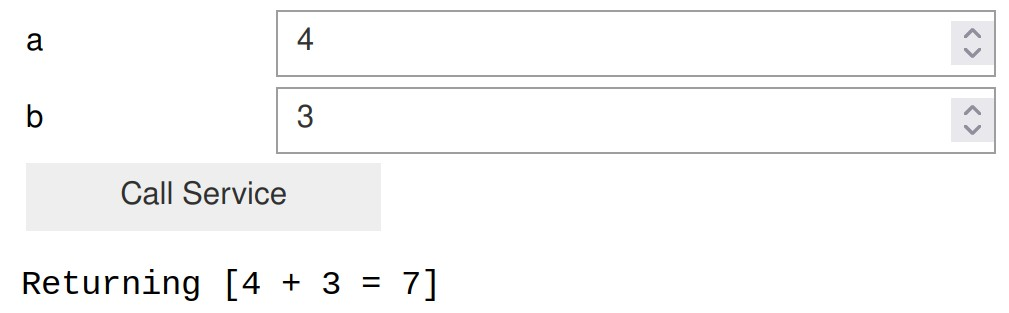
\includegraphics[width=10cm]{Images/01_clientWidget.jpg}
            \caption{Client Widget for an \texttt{AddTwoInts} message type}
            \label{fig:client}
        \end{figure}
    
        \noindent The client widget was also tested with other service message types such as the \texttt{Spawn.srv} from the \texttt{turtlesim} package. The client widget function successfully generated the expected results. The source code for the client function can be found \href{https://github.com/RoboStack/jupyter-ros/blob/master/jupyros/ros_widgets.py}{here}.
    
    \subsection{Pull Request}
    
        Once tested, a \href{https://github.com/RoboStack/jupyter-ros/pull/92}{pull request} was created. Additional changes were made after receiving feedback. This marked my first official contribution to \texttt{jupyros}.
        

\section{Turtlesim I}

    \subsection{ipycanvas Turtles}
        
        This project consisted of replicating the illustrious turtle simulation within a Jupyter notebook. The first step was to display a turtle image with the help of \href{https://ipycanvas.readthedocs.io/en/latest/index.html}{\texttt{ipycanvas}} library. All the turtle images can be found in the standard \texttt{turtlesim} package. 
        
        \begin{lstlisting}
from ipycanvas import Canvas
canvas = Canvas(width=1600, height=1200, layout={"width": "100%"})

# Water
canvas.fill_style = "#4556FF"
canvas.fill_rect(x=0, y=0, canvas.width, canvas.height)

# Turtle
turtle_canvas.draw_image(turtle_img, width=100)
        \end{lstlisting}
    
    \subsection{Random Turtles}
        Given that the \texttt{turtlesim\_node} displays a different turtle every time it is initialized, this behavior was imitated by storing the different turtle names in a list and selecting a random index to pull from that list.
        
        \begin{lstlisting}
turtle_path = turtle_img_path + 
              turtle_names[randint(0, len(turtle_names)-1)] + ".png"

turtle_img = Image.from_file(turtle_path)
        \end{lstlisting}
    
    \subsection{Rotating Turtles}
        
        The turtle images by default face "upward" or towards the top of the page. However, for an initial orientation of $0^\circ$ the turtles must face the right side of the page. To accomplish this, the canvas is first translated to the desired $x$ and $y$ position and then rotated by $\theta$ before drawing the turtle image. Once drawn, the canvas transformation is reversed.
        
        \begin{figure}[hb]
            \centering
            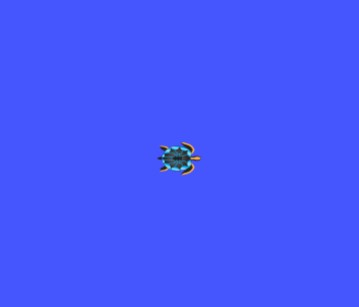
\includegraphics[width=7.5cm]{Images/01_spawn.jpg}
            \caption{Spawned turtle with an orientation of $0^\circ$}
            \label{fig:spawnTurtle}
        \end{figure}
    
        \begin{lstlisting}
canvas.translate(x, y)
canvas.rotate(radians(90))
canvas.draw_image(turtle_img, width=turtle_size)
canvas.rotate(radians(-90))
canvas.translate(-x, -y)
        \end{lstlisting}
        

        
        \noindent It must be noted that in the canvas coordinate system the $z-$axis points into the page, whereas, in the \texttt{turtlesim} coordinate the $z-$axis points in the opposite direction out of the page. The result from spawning a turtle in the middle of the canvas with an initial orientation of $0^\circ$ can be observed in Figure \ref{fig:spawnTurtle}.
    

    
    \subsection{Animating Turtles}
    
        The next step in the process was to create an animation function to move the turtle around the canvas. \texttt{ipycanvas} already provides the necessary tools for creating an \href{https://ipycanvas.readthedocs.io/en/latest/animations.html}{animation}, however, this created some issues with flickering of the image since the canvas was fully cleared during each iteration. To speed up the animation and to avoid the flickering effect, a \texttt{MultiCanvas} approach was used. The canvas consisted of four layers: the background, the path, and the last two for turtle motion. In this manner, the background and path can remain static while the turtle image is cleared only when there is another turtle image already drawn.
    
    \subsection{Tracing a Path}
    
        Lastly, the path the turtle traverses was created by a series of markers. Each time the turtle moves to a new position, a small circular marker is drawn at the coordinates of the new position. Because the canvas is multi-layered, the canvas where the markers are placed is never cleared, thus, they form a path as the turtle moves around the canvas. The results of the animation are shown in Figure \ref{fig:dottedPath}.
    
        \begin{figure}[hb]
            \centering
            \begin{subfigure}{.45\textwidth}
                \centering
                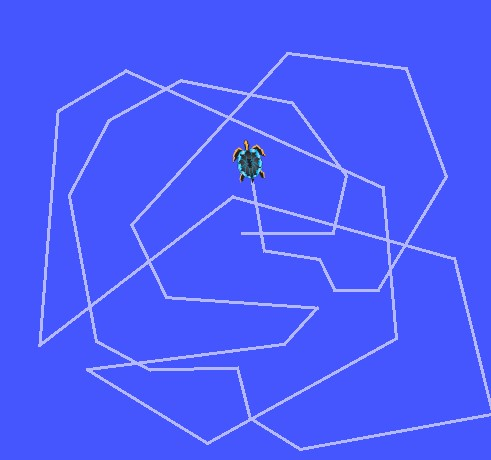
\includegraphics[height=6cm]{Images/01_realPath.jpg}
                \caption{Turtlesim original path}
                \label{fig:realPath}
            \end{subfigure}%
            \begin{subfigure}{.55\textwidth}
                \centering
                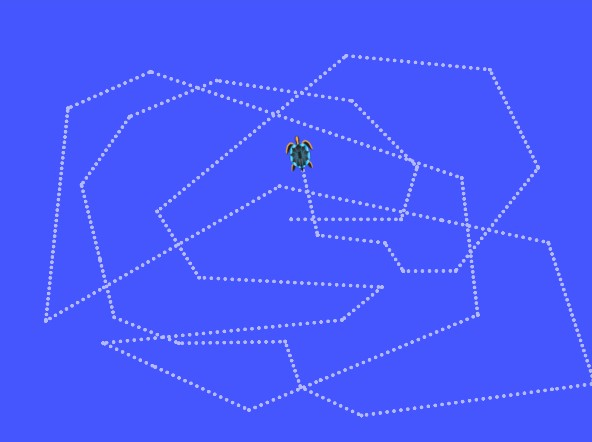
\includegraphics[height=6cm]{Images/01_path.jpg}
                \caption{Turtle path drawn with canvas markers}
                \label{fig:dottedPath}
                \end{subfigure}
                \caption{Comparison of the turtle path of ROS Turtlesim and the turtle path drawn with \texttt{ipycanvas}}
            \label{fig:comparePath}
        \end{figure}
    
\section{Future Work}

    The next step for this project is to create a turtle widget class. This will allow the storage of important information about the turtle such as the turtle image, the turtle's name, and its current position on the canvas. By having access to the turtle's position, the canvas path markers can be replaced with lines which will more closely resemble the original \texttt{turtlesim} path.




